\chapter{Implementation}
This implementation chapter covers key architecture aspects and the reasoning behind design decisions made while implementing the speech recognition system. 

\section{Loading data and feature extraction}
During system training as well as decoding usage at later stages, an infrastructure must be in place to load and process the input data. In the training phase the target data must be loaded, normalized, encoded and made available to the optimization algorithm in the correct form. The shape and encoding of the targets depends on the algorithm used. Connectionist temporal classification requires a blank output label for example, which listen attend and spell does not need.
The code written to handle the data preprocessing fulfills these requirements.\footnote{Its development history as well as the process of harminizing the interfaces of the thesis code with the rest of the toolbox is recorded in the project git branch at \url{https://github.com/vrenkens/tfkaldi/commits/las}.}

\section{Efficient sequence to sequence implementations}
When working with sequence to sequence methods such as CTC, data processing problems arise naturally. For efficiency reasons it is beneficial to work with
fixed size data tensors. However the number of frames varies significantly between utterances. The same holds true for the target lengths. In order to still be able to work with fixed size tensors, the inputs and targets must be padded with zeros or unknown tokens to fill up the length differences.
In order to keep the speed benefit of working with tensors it is important to
keep track of the sequence lengths of every individual utterance.
The sequence length information must be used to avoid actually processing any of the padded data, that the tensors where filled up with in order to allocate memory faster.
The listener produces a three dimensional logit tensor of size $[B, T, F]$, where $B$ denotes the batch size, $T$ the largest occuring frame number and $F$ the feature dimension size. When implementing the output layer the na\"{\i}ve approach would be to loop over the time dimension, and evaluate the linear layer T times with a $B$ times $F$ matrix. Which is simple to implement but very inefficient. Instead the sequence information should be used to remove the padding and concatenate the batch dimension into a matrix $\mathbf{X}$ of size $[S, F]$, where $S$ denotes the sum of all sequence lengths. The linear layer can then be evaluated as:
\begin{equation}
\mathbf{W}\mathbf{X} + \mathbf{b} = \mathbf{R}
\end{equation}
The result matrix $R$ can then be converted back into a padded tensor using the sequence length information one more time.
An alternative approach which avoids reshaping is to implement a linear recurrent network cell with a state size of zero and use dynamic unrollings the evaluate the linear layer. The resulting memory requirements and speed are comparable.

\section{Design of the BLSTM-CTC model}
Sequence labeling using confectionist temporal classification happens in two phases. First BLSTM layers compute annotations based in the input vectors. These annotations are then handed to a CTC layer which runs the annotations trough a softmax to produce normalized label probabilities and computes the loss during training or searches trough the probability distributions during decoding. 
The BLSTM-CTC implementation reflects this procedure by splitting the BLSTM layers as well as the training and decoding code into model, trainer and decoding classes. \footnote{It was not necessary to implement CTC decoding. Tested code is already available at \url{www.tensorflow.org/api_docs/python/nn/connectionist\_temporal\_classification\_\_ctc\_}} 



\section{Implementing Listen attend and Spell}
The listen operations computing the high level feature matrix $\mathbf{H}$ can be completed independently before the attend and spell code is run. All listening related code has therefore been grouped in a Listener class, all attend and spell related functions are grouped in a speller class.

\subsection{The Listener}
The Listener consists of an initial bidirectional long short term memory layer (BLSTM), followed by pyramidal LSTM (PLSTM ). The plstm layer compresses the time dimension as described in chapter \ref{subsec:Listener}. The compression has been implemented by looping trough the hidden output of the previous layer in time and concatenating every second vector with the one before it. Every PLSTM layer therefore halves the time dimension and produces an output of two times the state size of it's LSTM cells. 
For use with CTC a liner output layer can optionally be added to the listener, which maps the output from two times the state size to the number of required labels. 

\subsection{The Speller}
Based on the high level features $\mathbf{H}$ computed by the listener the speller evaluates an internal attention mechanism. This mechanism which can be interpreted as a learned sliding window. The speller learns where to place this window based on the decoder state $\mathbf{s}_i$. This state therefore represents a query, which asks the attention mechanism to provide certain information. This query in turn is computed by the spellers internal RNN.  Using the attention factors a context vector $\mathbf{c}$ is computed, which together with the state is used to assign a label. 
The attention computations described above and in more detail in \ref{subsec:AttendAndSpell}, do only depend on data available at the current time and previously computed values. The spellers key functions can therefore be implemented within an RNN cell. The state of this augmented RNN cell at decoding time step $i$ is given by:
\begin{align}
\text{state} =  [\mathbf{y}_{i-1}, \mathbf{s}_{i-1}, \mathbf{c}_{i-1}]
\end{align}
The one hot encoded previous label is denoted by $\mathbf{y}$ the decoder state by $\mathbf{s}$ and context by $\mathbf{c}$.
\begin{figure}
\centering
\includestandalone{tikz/asCellType1}
\caption{Schematic of the attend and spell cell components.}
\label{fig:asCell}
\end{figure}
A visualization of the attend and spell cell implementation is shown in figure~\ref{fig:asCell}. The blue box surrounding the attend and spell represents a \texttt{while} or \texttt{for} loop. The loop type depends on whether the speller is run in training or decoding mode. 
The ground-truth labels are known during training. The attend and spell cell must therefore be evaluated until a sequence of the same length as the ground-truth has been obtained. Taking knowledge of the target sequence length into account the unrolling can be done in a \texttt{for} loop. 
Running in decoding mode is harder, because the length of the sequence the model will assign to the input is unknown. 

\subsubsection{Design of the decoding loop logic}
The attend and spell cell must be evaluated until it produces an end of sentence token or an iteration maximum has been reached. The system should be able to decode multiple sequences in parallel. In order to keep track of the active sequences a done vector $\mathbf{d}$ is introduced.  $\mathbf{d}$ contains one entry per sequence, each entry should contain \texttt{True} if an \texttt{<eos>} token has been produced during decoding of the corresponding input and \texttt{False} if not. 
To achieve the desired behavior the following loop logic has been devised:
\begin{lstlisting}[language=python]
while keep_working:
	not_done_count = reduce_sum( logical_not( d ))
	done = equal(not_done_count, 0)
	stop_loop = logical_or(done, greater(time, max_steps))
	keep_working = logical_not(stop_loop)
\end{lstlisting}
The pseudocode above uses relies on the mask $\mathbf{d}$ and an upper step limit to check if the while loop should continue running. In order to implement decoding efficiently inside of a graph it is important to keep track of the sequence lengths. The decoding loop implementation does this when it determines the done mask $\mathbf{d}$. During every iteration the loop body updates the sequence lengths with the current decoding time, unless $\mathbf{d}$ contains \texttt{True} at the position corresponding to the current utterance.
\begin{lstlisting}[language=python]
     decoded = decode(logits)
     mask = tf.equal(decoded, <eos>)

     time_vec = ones(self.batch_size)*(time+1)
     sequence_lengths = select(d,
                               logits_sequence_length,
                               time_vec)
     d = logical_or(mask, d)
\end{lstlisting}
The code listing above updates $\mathbf{d}$ after the sequence lengths have been updated, because the \texttt{<eos>} token should be recorded as well. It is assumed that the decoded function returns a one hot vector and \texttt{<eos>} represents an encoded end of sentence token. $\mathbf{d}$ is initialized to \texttt{False} for all sequences. 

\subsubsection{Cell efficiency improvements}
In figure~\ref{fig:asCell} the feature net output $\psi(\mathbf{h_u})$ is evaluated inside the cell. While closely following the equations in \cite{Chan2015}, evaluating the feature net inside the cell means accessing $\mathbf{H}$ and evaluating an MLP at every decoding time step. Instead the $\psi(\mathbf{h_u})$ can be computed outside of the cell ahead of decoding time and a matrix $\hat{\mathbf{H}}$ consisting of $\psi(\mathbf{h_u})$ for all $u$ is used inside the cell.
Furthermore all computations have been implemented using matrix tensor multiplication functions instead of for loops, which yields large performance increases. 
\begin{figure}
\centering
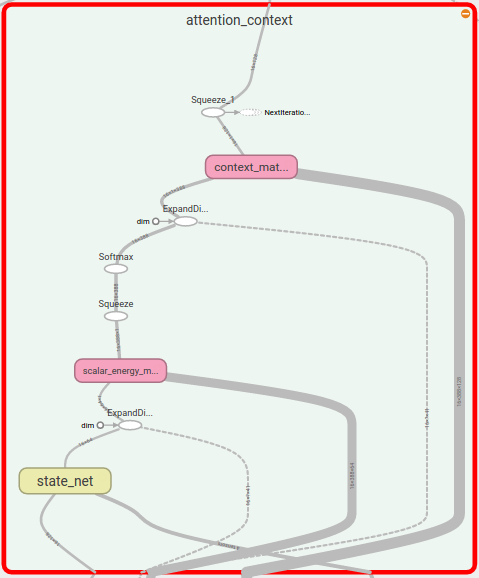
\includegraphics[width=0.49\linewidth]{../png/attention_context}
\caption{Tensorboard visialization of the attention context computations.}
\label{fig:attention_context}
\end{figure}
Figure~\ref*{fig:attention_context} shows a tensorboard\footnote{\url{https://www.tensorflow.org/versions/master/how_tos/graph_viz/}} visualization of the attention computation. The rose colored blocks represent matrix multiplications.

